% Chapter Electrodes

\chapter{Scanning over the Parameters of the Design Simulation} % Main chapter title

\label{ChapterElectrodesScan} % Change X to a consecutive number; for referencing this chapter elsewhere, use \ref{ChapterX}

%----------------------------------------------------------------------------------------
%	BEGING CHAPTER
%----------------------------------------------------------------------------------------

% Intro
This section presents the results of scanning over the parameters of the PL38 and the FID38 design electrostatic simulation. These scan aims at understanding the influence  of each parameter on the ionization channel operation. All the design parameters were introduced in the previous chapter \ref{ChapterElectrodes}. For a prompt description of the parameters of the PL38 design, the reader should refer to the table \ref{tab:pl38-default-parameters} and the scheme \ref{fig:pl38-scheme}. For parameters relative to the FID38 design, the reader should refer to the table \ref{tab:fid38-default-parameters} and the scheme \ref{fig:fid38-scheme}. 
This chapter first introduces the methodology used for the parametric scan. It follows with a study of the impact of design parameters shared by both the PL38 and the FID38 design. Then are presented the studies on the influence of parameters specific to the PL38 design and the FID38 design.


\section{Parametric Scanning Methodology}

As discussed in the previous chapter \ref{ChapterElectrodes}, the performances of the ionization channel mainly hold in a good charge collection and the a low baseline resolution.
% Capacitance metric
In order to have a low baseline resolution, the ionization channel should present a low level of noise and the high signal sensitivity. In the paragraph \ref{par:ion-resolution-calculation}, the resolution is deduced from the computation of the signal sensitivity and the noise level of the two detectors designs. These computation are based on the Maxwell matrix capacitance obtained from the electrostatic simulation of PL38 and FID38 designs. Scanning the multi-dimensional parameter space of the two detector design does not allow for this resource-intensive computation chain. However, it was shown in \ref{par:ion-resolution-calculation}, that the baseline resolution of the ionization channel roughly follows a linear law with the terms of the Maxwell capacitance matrix. Tempering this observation with further insights presented in the previous chapter \ref{ChapterElectrodes}, the Maxwell and mutual capacitance terms can be used as a valid metric when discussing the influence of the design parameters on the detector resolution.
% Fiducial volume metric
The charge collection is broad expression covering the fiducial volume, the trapping rate and the signal generation by the drifting electric charges. While the real fiducial volume can only be accessed through experimentation, it can be inferred from the knowledge on the electric charge drifting in germanium (see paragraph \ref{par:charge-drifting}) and the theoretical fiducial volume obtained with electrostatic simulation (see paragraph \ref{par:fiducial-volume}).
% enorm metric
A precise value for the electric charge trapping rate is difficult to forecast in the bulk. However, it is known that region of the crystal with low magnitude of electric field demonstrate a higher propensity to charge trapping. The next chapter \ref{ChapterElectrodeExperimental} demonstrates using the analysis of the RED80 data, that over a critical threshold of $|\vec{E}|=\SI{0.1}{\volt\per\centi\meter}$ (to be verified!!!), the trapping rate is constant. %Thus, tracking the volume fraction displaying a lower electric field norm should 
% weighting potential metrix
On further notice concerning the signal generation, the electric charge conservation equation \ref{eq:charge-conservation} depends on the quality of the Faraday cage formed by the aluminium electrodes which is quantified by the total weighing potential (TWP) in paragraph \ref{par:weighting-potential}. A low TWP coupled with a high trapping rate could result in substantial fraction of the events to be discarded or worse, ill-reconstructed, in the analysis.

% Conclusion on Metrics
On those grounds, a metric is established for the study of the design parameters influence. For each scanned configuration, the variations over the terms of the Maxwell $\bm{C}$ and mutual $\bm{C}^m$ capacitance matrices, the fiducial volume fraction $\%_{fid}$, the electric field norm $|\vec{E}|$ as well as the weighting potentials $\Phi_X$ are documented. In some cases, the variation over the considered capacitance terms $C_{XX}$ is more appropriately illustrated with a ratio:
\begin{equation}
\frac{C_{XX}\left(p=x\right)}{C_{XX}\left(p=p_0\right)}
\end{equation}
where $p$ is the scanned parameter, $p_0$ a reference value (usually the default value) and $x$ the scanned value. As the electric field norm $|\vec{E}|$ and the weighting potential $\Phi_X$ are scalar fields and their variations are generally homogeneous in the crystal volume, it is challenging to propose a universal scalar quantity for discussion. Consequently, the illustration and features of these fields used for the scan interpretation are specific to the considered parameter and selected at the best of the authors' discretion.

% Multi dimension and scan over one parameter
For each detector designs, the configuration of the electrostatic simulation is set by several parameters. Thus, this study calls for a multi-dimensional scan over the design parameters and could even result in a semi-automated optimization of the design like what is achieved for the heat channel in chapter \ref{Chapters/ChapterEthem}. Nevertheless, the performance of the ionization channel cannot be gauged with a single quantity and invalidate such a ionization channel design optimization. As such, the study presented in this chapter focuses on understanding the influence of each parameter by carrying multiples one-dimensional scans. Only one parameter is scanned over at a time with all the other parameters sets to default values. Hence, the control quantities resulting from a scan can be compared to the default design value which was discussed in the previous chapter \ref{ChapterElectrodes}.
Although simpler, this method explicitly omits a massive portion of the parametric space. This introduces the risk of scanning far from an optimal configuration and collecting only marginal insights on the ionization channel design. However, this risk is heavily mitigated by the fact that the default configuration of the PL38 and the FID38 detectors designs presented in the chapter \ref{ChapterElectrodes} are the product of a manual optimization inspired by the whole thesis work on ionization channel.


\section{Common Parameters}

In this section, each paragraph presents the scan over a parameter common to the PL38 and the FID38 detector designs. These common parameters are namely the thickness of the aluminium deposit $h_{Al}$, the distance between the grounded chassis and the germanium crystal $d_{Cu}$, the bias voltage $V_{bias}$ and the polarization symmetry $S_{bias}$.


\subsection{Aluminium Deposit Thickness, $h_{Al}$}
% Moving this subsection to the previous chapter for error estimation ?

The thickness of the aluminium electrodes used in the COMSOL simulation is noted $h_{Al}$. It is not in itself a design parameter as the actual thickness depends on the fabrication process and is usually of about \SI{50}{\nano\meter}. This value is much lower than any geometric feature in the COMSOL simulation which, if implemented as is, would induce a complex meshing and a long simulation time. As to keep the simulation resource cost reasonable, the electrostatics simulation are ran with a greater thickness than in reality at the expense of small supplementary errors. For the FID38 geometry, the electrostatic simulation is ran multiple times scanning over the electrode thickness $h_{Al}$. The table \ref{tab:al-thickness} presents for each value of $h_{Al}$ the number of triangles in the mesh, the diagonal Maxwell capacitance of top collect (B) electrode $C_{BB}$ and the relative error on this capacitance. The reference for the error calculation is considered to be the capacitance computed for the lowest value $h_{Al}=\SI{0.1}{\micro\meter}$.

\begin{table}[ht]
\centering
\begin{tabular}{S|r|r|S}
{$h_{Al}/\si{\micro\meter}$} & {\# Triangles} & {$C_{BB}/\si{\pico\farad}$} & {Relative Error / \si{\percent}} \\ \hline \hline
100 & 7413   & 20.419 & 7.3  \\ \hline
30  & 13959  & 19.560 & 2.8  \\ \hline
10  & 22504  & 19.232 & 1.1  \\ \hline
3   & 34745  & 19.102 & 0.4  \\ \hline
1   & 58815  & 19.053 & 0.1  \\ \hline
0.3 & 76637  & 19.034 & 0.02 \\ \hline
0.1 & 106057 & 19.029 & 0    \\
\end{tabular}
\caption{Scanning over the electrode thickness $w_{Al}$ of the FID38 design. The control values are the number of triangles in the mesh, the first diagonal term of the Maxwell capacitance matrix and the relative error on the capacitance calculation with the lowest thickness $h_{Al}=\SI{0.1}{\micro\meter}$ chosen as reference.}
\label{tab:al-thickness}
\end{table}

As expected from simulating thin electrodes, the number of triangles composing the mesh is drastically increased. Also, as the electrodes presents a lower area, their capacitance is slightly lowered, eventually capping for the lowest thickness values. In other words, the computation of the capacitance term is getting more precise with decreasing electrode thickness. A trade-off is selected at $h_{Al}=\SI{1}{\micro\meter}$ with a relative error of \SI{0.1}{\percent}. Indeed, this quantity is reminiscent of the relative error of \SI{0.08}{\percent} induced by the chosen mesh scale "Fine" presented in paragraph \ref{par:mesh-scale}.


\subsection{Chassis Distance, $d_{Cu}$}

The chassis distance $d_{chassis}$ is the distance between the grounded copper chassis and the planar and lateral faces of the germanium crystal. Its default value is set to \SI{3}{\mm} for both the PL38 and the FID38 design. The scan is performed on a logarithmic scale from \SIrange{0.1}{10}{\mm}. The results are presented in the figure \ref{fig:capacitance-fiducial-cu-distance-pl38} for the PL38 design and in the figure \ref{fig:capacitance-fiducial-cu-distance} for the FID38 design. Both figures display the terms of the Maxwell $\bm{C}$ and mutual capacitance matrix $\bm{C}^m$ along with the fiducial volume fraction $\%_{fid}$ as functions of the chassis distance $d_{Cu}$ for their respective detector design. Additionally, percentiles $f_x$ of the electric field norm $\| \mathbf{E} \|$ distribution are plotted for the FID38 design.

\begin{figure}
\centering
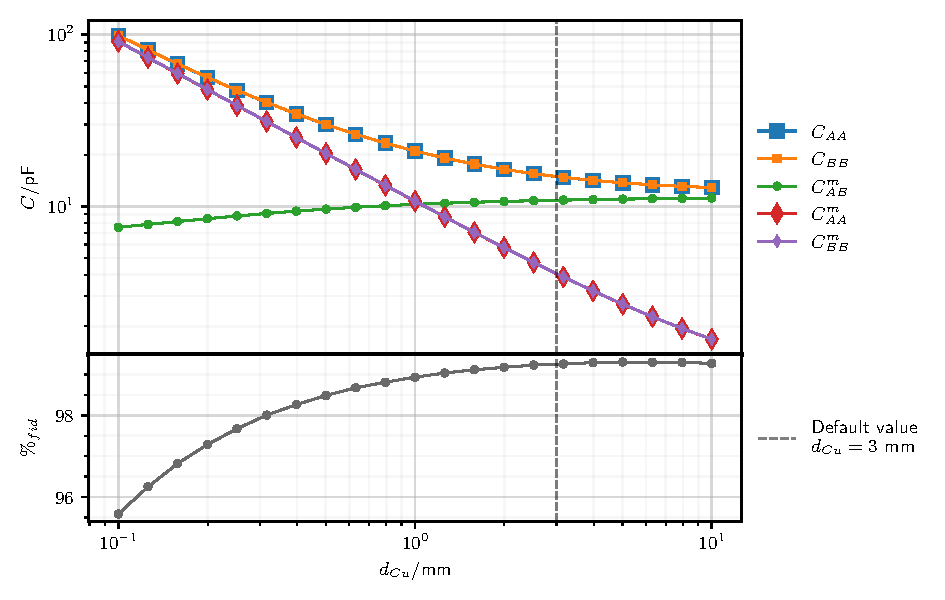
\includegraphics[scale=1]{Figures/ElectrodesScan/capacitance_fiducial_cu_distance_pl38.pdf}
\caption{Scan over the chassis distance $d_{Cu}$ for the PL38 design. The Maxwell and mutual capacitance terms and the percentage of fiducial volume $\%_{fid}$ are plotted separately. The default value $d_{Cu}=\SI{3}{\mm}$ is represented by the dashed vertical line. Error bars are smaller than the marker size.}
\label{fig:capacitance-fiducial-cu-distance-pl38}
\end{figure}

\begin{figure}
\centering
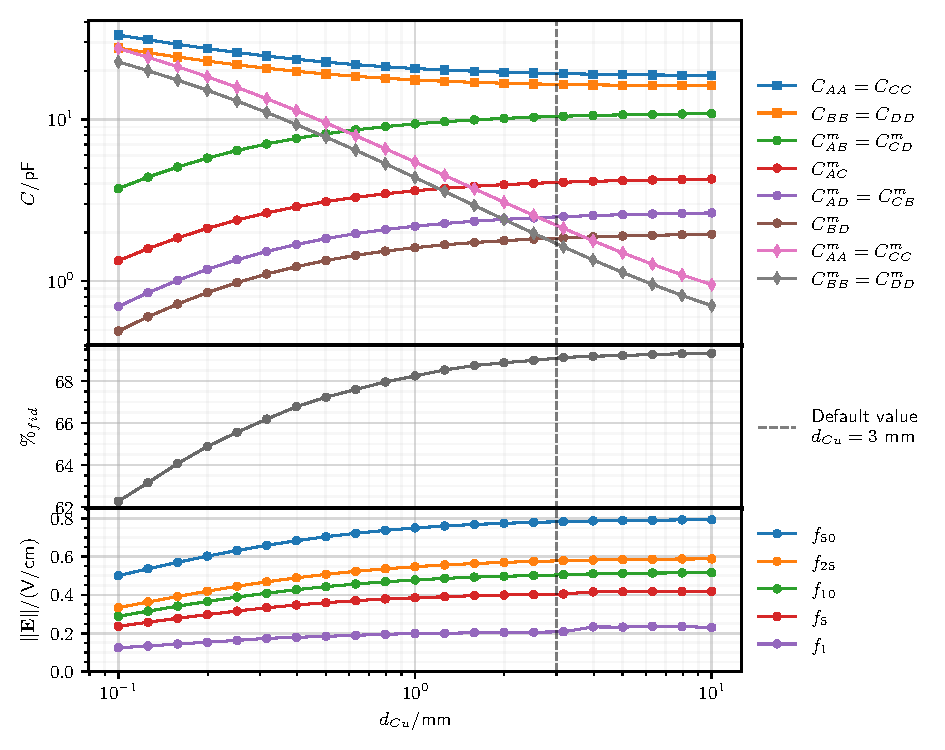
\includegraphics[scale=1]{Figures/ElectrodesScan/capacitance_fiducial_cu_distance.pdf}
\caption{Scan over the chassis distance $d_{Cu}$ for the FID38 design. The Maxwell and mutual capacitance terms, the percentage of fiducial volume $\%_{fid}$ and some percentiles $f_x$ of the electric field norm $\| \mathbf{E} \|$ are plotted separately. The default value $d_{Cu}=\SI{3}{\mm}$ is represented by the dashed vertical line. Error bars are smaller than the marker size.}
\label{fig:capacitance-fiducial-cu-distance}
\end{figure}

% Common
We can first discuss the trends common to both design. 
% Fiducial
The percentage of fiducial volume $\%_{fid}$ increases with the chassis distance $d_{Cu}$ and reaches a plateau. This effect is slight in the case of the PL38, with a gain of about \SI{2.75}{\percent} between the extremes values of $d_{Cu}$. This is explained by a contraction of the exiting streamlines ragions on the lateral surfaces and under the central NTD hole. In the case if the FID38, the effect is more significant with a growth of about \SI{6.5}{\percent} from \SIrange{e-1}{e1}{\mm}. The reason is the reduction of the depth of the veto regions inducing a raise in fiducial volume.
% Capacitance
For both detector design, the non-diagonal term of the mutual matrices $C_{XY}^m$ increases to reach a plateau with the chassis distance while the self-capacitance $C_{XX}$ decreases. As a result, the diagonal terms of the Maxwell capacitance matrix $C_{XX}$ diminishes following two emerging regimes. In the first regime for low chassis distance ($d_{Cu} \leq \SI{1}{\mm}$ for PL38 and $d_{Cu} \lesssim \SI{0.6}{\mm}$ for FID38), the self-capacitance term dominates the calculation of the diagonal Maxwell terms. Indeed, with a very close chassis, the capacitive coupling between the ground and the electrodes overshadows the other couplings. As the chassis moves away, the calculation of the diagonal Maxwell terms is dominated by the inter-electrodes coupling terms $C_{XY}^m$. 
% TWP
The heightened influence of the copper chassis is also observed for the total weighting potential (TWP). On the surfaces of the detectors bare of aluminium electrodes, the TWP is as low as $0.3$ for minimal $d_{Cu}$ as the drifting electric charges induce a lot of signal on the close electric ground. For the maximal value of $d_{Cu}$, the TWP reaches $0.975$ on the surface as the copper chassis is too far away from the drifting charges to collect a significant fraction of the signal.

% Enorm
The behavior of the magnitude of the electric field $\| \mathbf{E} \|$ differs between the PL38 and FID38 designs. For the former, the magnitude is almost constant in the crystal save for slight variation on the bare lateral surface and the under the central NTD hole. For the latter design, the last subplot of the figure \ref{fig:capacitance-fiducial-cu-distance} shows a global increase of the electric field norm with the chassis distance as all the percentiles of the distribution are concerned by the growth.
{\color{red} [Comparison to enorm threshold, to do later.]}

% Conclusion
The results points towards better detector performances with a high chassis distance. Indeed, for both designs, the fiducial fraction increases, the capacitance terms globally decreases, the total weighting potential tends to 1 and the electric field norm even grows for the FID38. The constraint on the chassis distance is imposed by the size of the Teflon clamps holding the crystal inside the chassis and the maximal dimensions of the detector load in the cryostat. As all the control quantities asymptotically reach a plateau with high chassis distance starting from $d_{Cu} \gtrsim \SI{1}{\mm}$, the value $d_{Cu} = \SI{3}{\mm}$ is chosen for the detector designs.

% bonus observation
%- PL38: Confirmed by the low enorm region under the central ntd hole going deeper into the crystal


\subsection{Bias Voltage, $V_{bias}$}

The bias voltage $V_{bias}$ corresponds to the voltage between the two main electrodes of the detectors.
By default, it set to 2V. The scan is performed on a logarithmic scale from \SIrange{e-1}{e1}{\volt}. The results are presented in the figure \ref{fig:capacitance-fiducial-V-bias-pl38} for the PL38 design and in the figure \ref{fig:capacitance-fiducial-V-bias} for the FID38 design. Both figures display some percentiles $f_x$ of the electric field norm $\| \mathbf{E} \|$ distribution.

\begin{figure}
\centering
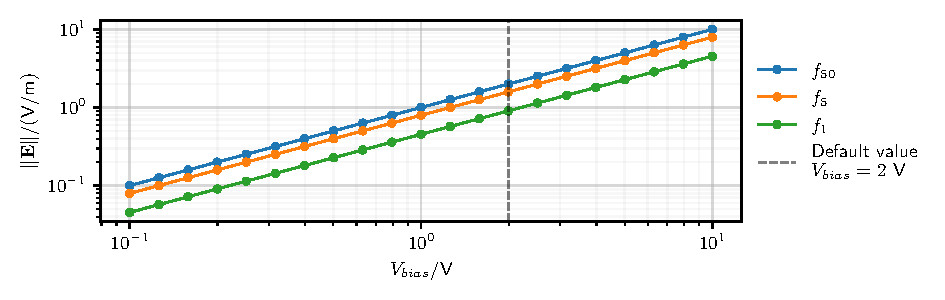
\includegraphics[scale=1]{Figures/ElectrodesScan/capacitance_fiducial_V_bias_pl38.pdf}
\caption{Scan over the bias voltage $V_{bias}$ of the PL38 design. Some percentiles $f_x$ of the electric field norm $\| \mathbf{E} \|$ are plotted. The default value $V_{bias}=\SI{2}{\volt}$ is represented by the dashed vertical line. Error bars are smaller than the marker size.}
\label{fig:capacitance-fiducial-V-bias}
\end{figure}

\begin{figure}
\centering
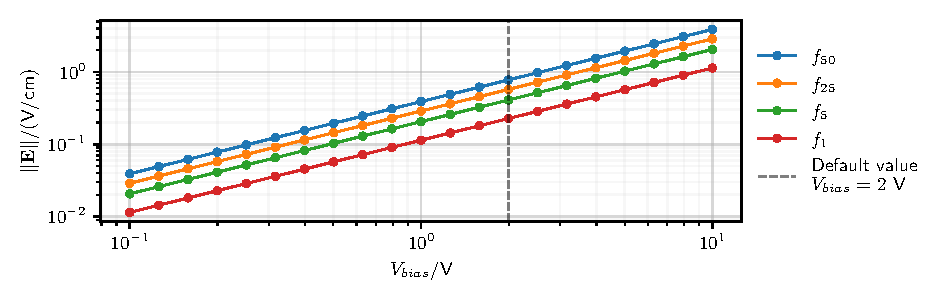
\includegraphics[scale=1]{Figures/ElectrodesScan/capacitance_fiducial_V_bias.pdf}
\caption{Scan over the bias voltage $V_{bias}$ of the FID38 design. Some percentiles $f_x$ of the electric field norm $\| \mathbf{E} \|$ are plotted. The default value $V_{bias}=\SI{2}{\volt}$ is represented by the dashed vertical line. Error bars are smaller than the marker size.}
\label{fig:capacitance-fiducial-V-bias-pl38}
\end{figure}

% unaffected
As the bias voltage solely affect the polarization of the electrodes, the capacitance terms and the total weighting potential are unaffected for this scan. Moreover, according to the equations \ref{eq:voltage-bias-pl38} and \ref{eq:voltage-bias-fid38} , the electric potential of all the electrodes are proportional to the parameter $V_{bias}$. As such, the electric field lines as well as the theoretical fiducial volume are unchanged for this scan. 
% enorm
For both designs, the electric field in the crystal scales proportionally with the voltage bias $V_{bias}$. At lower voltage, the magnitude could be lower than the critical threshold.
{\color{red} [Comparison to enorm threshold, to do later.]}

% Conclusion
A high magnitude is preferred for a good charge collection. However, according to the discussion in the paragraph \ref{par:double-energy-measurement}, a low voltage bias yields a better discrimination between electronic and nuclear recoils thanks to the lowered Luke-Neganov effect. Balancing this two aspect, we choose the lowest bias voltage possible while keeping a reasonable (???) fraction of the volume above the critical magnitude threshold. For now, the bias voltage $V_{bias} = \SI{2}{\volt}$ is selected for the PL38 and the FID38 designs.


\subsection{Polarization Symmetry, $S_{bias}$}

The polarization symmetry $S_{bias}$ is a parameter used to set the global symmetry of the polarization for the PL38 according to equation \ref{eq:symmetry-pl38} and FID38 according to equation \ref{symmetry-fid38}. The scan is performed on a linear scale from $0$ to $1$, with $S_{bias}=0.5$ fixing a symmetric polarization and being the default value for this parameter. For the PL38 design, the fiducial volume percentage $\%_{fid}$ and some percentiles $f_x$ of the electric field norm $\| \mathbf{E} \|$ distribution are plotted in the figure \ref{fig:capacitance-fiducial-V-symmetry-pl38}.

\begin{figure}
\centering
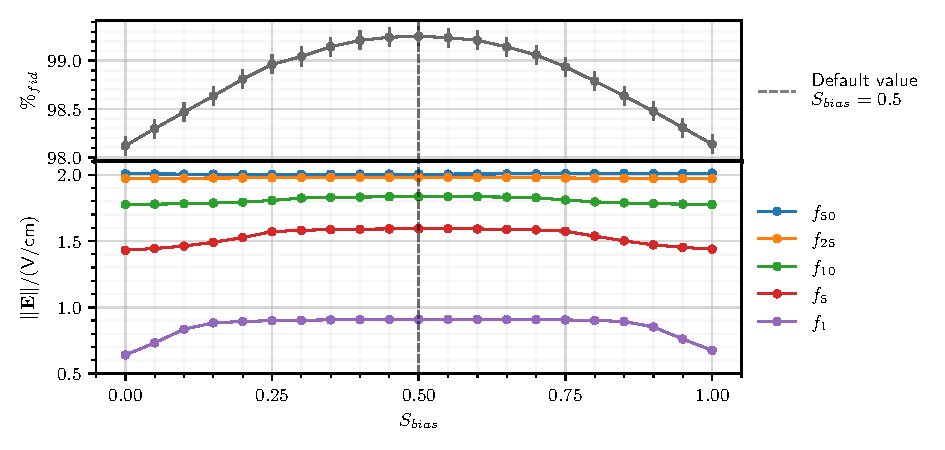
\includegraphics[scale=1]{Figures/ElectrodesScan/capacitance_fiducial_V_symmetry_pl38.pdf}
\caption{Scan over the polarization symmetry $S_{bias}$ of the PL38 design. The percentage of fiducial volume and some percentiles $f_x$ of the electric field norm $\| \mathbf{E} \|$ are plotted. The default value $S_{bias}=\SI{0.5}{}$, corresponding to the symmetric polarization, is represented by the dashed vertical line. Error bars are smaller than the marker size.}
\label{fig:capacitance-fiducial-V-symmetry-pl38}
\end{figure}

% unaffected
As the polarization symmetry parameter $S_{bias}$ solely affect the electric potential of the electrodes, the capacitance terms and the total weighting potential are unaffected in both designs for this scan. 
% FID38
In the case of the FID 38 design, the fiducial volume and the electric field norm distribution are unchanged. With varying $S_{bias}$, variations in the electric potential are plenty in the vacuum surrounding the crystal and only negligible changes in the shape of the electric field lines are observed inside the germanium crystal near the equator.

% PL38
The symmetry parameter $S_{bias}$ has more influence for the PL38 design. As shown in the figure \ref{fig:capacitance-fiducial-V-symmetry-pl38}, asymmetrical polarization feature a slightly lowered fiducial volume percentage compared to the optimum for the symmetrical polarization. As the electric potential of the top or bottom electrode goes to \SI{0}{\volt}, same as the grounded copper chassis, more field lines near the surface are exiting the crystal. Additionally, the electrode with nullified potential sees its low electric field magnitude corner gain in volume. As a result, the magnitude distribution over the crystal volume is broaden towards lower value as shown by the significant decrease of the percentiles $f_1$ and $f_5$ for asymmetrical polarization value.
The influence of the parameter $S_{bias}$ is mitigated by the lateral corners of the electrodes and theri length $L_{lat}$. The observed trends are expected to be exacerbated for PL38 designs with lower or non-existent lateral corners.
{\color{red} [Comparison to enorm threshold, to do later.]}

% Conclusion
It seems that the effects of the parameter $S_{bias}$ are minors. While there exists an optimum in performances for a symmetric polarization at $S_{bias}=\num{0.5}$, operating the PL38 and FID38 with asymmetrical electrode potential is viable and could potentially alleviate some future issues with the influence of the NTD thermal sensor on the electric field. 


\section{Specific to PL38}

This section is attributed to the PL38 design. Each paragraph presents the scan over a parameter. They are namely the radius of the central NTD hole $r_{center}$ and the length of the lateral corners of the electrodes $L_{lat}$.


\subsection{Radius of the central hole for the NTD, $r_{center}$}

In order to glue the NTD thermal sensor on bare germanium, a central hole of radius $r_{center}$ is made of the top electrode of the PL38 design. By default,the radius is set to $r_{center} = \SI{1.5}{\mm}$ to fit a standard \SI{2 x 2}{\mm} NTD thermal sensor. Another significant radius is $r_{center}=\SI{3}{\mm}$ which can fit a larger \SI{4 x 4}{\mm} NTD thermal sensor. The scan is performed on a linear scale from \SIrange{0}{5}{\mm}. The results of the scan are presented in the figure \ref{fig:capacitance-fiducial-r-center-pl38} as graphs of the fiducial volume percentage and capacitance term ratio.

\begin{figure}
\centering
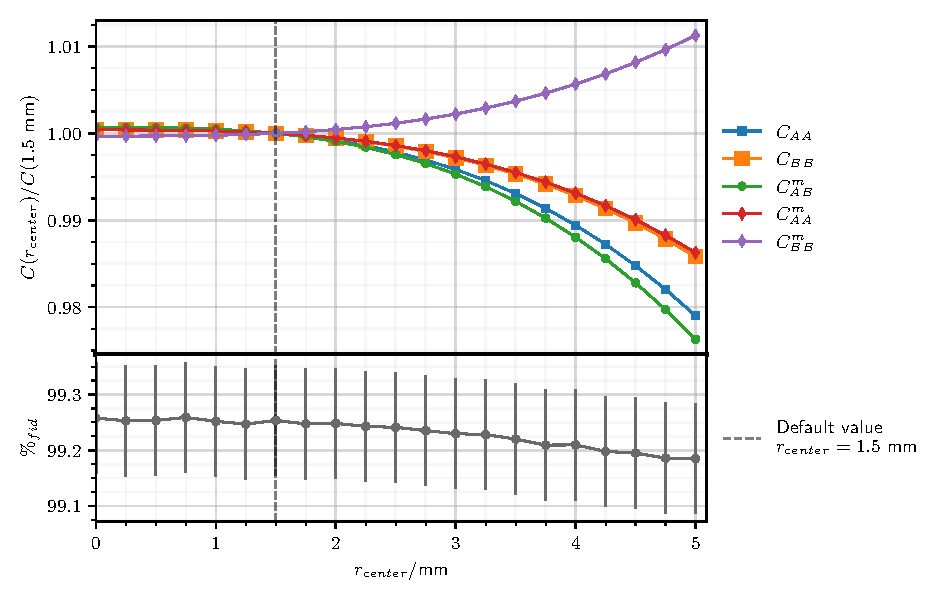
\includegraphics[scale=1]{Figures/ElectrodesScan/capacitance_fiducial_r_center_pl38.pdf}
\caption{Scan over the radius of the central NTD hole $r_{center}$ of the PL38 design. The Maxwell and mutual capacitance terms ratio and percentage of fiducial volume are plotted. The capacitance term ratio is calculated with the default capacitance value as denominator. The default value $r_{center}=\SI{1.5}{\mm}$ is represented by the dashed vertical line. Error bars for the capacitance ratio are smaller than the marker size.}
\label{fig:capacitance-fiducial-r-center-pl38}
\end{figure}

% Capacitance
The figure shows that all the capacitance terms decreases with $r_{center}$ except for the self-capacitance of the bottom electrode $C_{BB}^m$. Indeed, as the hole in the top electrode $A$ grows, the bottom electrode $B$ faces an increasing area of grounded chassis through the hole. On the contrary, as the hole grows in size, the top electrode $A$ lose in area thus reducing its coupling with the ground and the bottom electrode $B$. The inter-electrode coupling term $C_{AB}^m$ is dominant is the calculation of the diagonal Maxwell terms $C_{XX}$ and imposes its decreasing trend with $r_{center}$. One should note that the variations on the capacitance terms are inferior to \SI{3}{\percent} and thus almost negligible.
% Fiducial and enorm
The growing central hole in the electrode induces a greater low electric field magnitude region under it. Electric field lines are diverging from this low magnitude region resulting in a lower theoretical fiducial volume. However, according to the figure \ref{fig:capacitance-fiducial-r-center-pl38}, this reduction is almost negligible. Indeed, the change is located on the central axis of the crystal and affects a marginal fraction of the total volume. In line with this remark, the distribution of the electric field magnitude on the volume is negligibly affected by the scan over $r_{center}$. Even though the impacted volume is very low, the central hole creates a surface bare aluminium electrode with a very low electric field. As a result, recoils in this region should be prone to surface trapping. {\color{red} [Comparison to experiment with hole in electrode, NbSi ?]}
% TWP
As for the total weighting potential, there is a slight decrease on the surface in the central hole from $1$, with a non-existent hole, to \num{0.94}, with the largest value $r_{center}=\SI{5}{\mm}$.

% Conclusion
Although the performances of the ionization channel would be optimal with no central NTD hole, with $r_{center}\SI{0}{\mm}$, the variation on the control values are almost negligible. The trade-off presented by the parameter $r_{center}$ holds in a balance between a higher heat sensitivity with a NTD thermal sensor glued on bare germanium and a possible problematic charge collection under the central NTD hole. As a result, the lowest radius possible is favored for the designs. In the case of the standard \SI{2 x 2}{\mm} NTD thermal sensors, it corresponds to $r_{center}=\SI{1.5}{\mm}$.

% bonus observation
% In term of real fiducial volume, with this low e norm region with a bare germanium surface, we can expect recoil in this region to produce charges easily trapped on the surface, or with recombination problem.


\subsection{Corner length, $L_{lat}$}

The planar electrodes of the PL38 design extends on the lateral surfaces on a length $L_{lat}$ deemed corner length. The default value is $L_{lat} = \SI{2}{\mm}$. The scan is performed on a linear scale from \SIrange{0}{4.8}{\mm} (at a value of \SI{5}{\mm}, the top and bottom electrode would be touching). The results of the scan are presented in the figure \ref{fig:capacitance-fiducial-corner-length} as graphs of the terms of the Maxwell and mutual capacitance matrices, the percentage of fiducial volume and some percentiles of the electric field magnitude distribution.

\begin{figure}
\centering
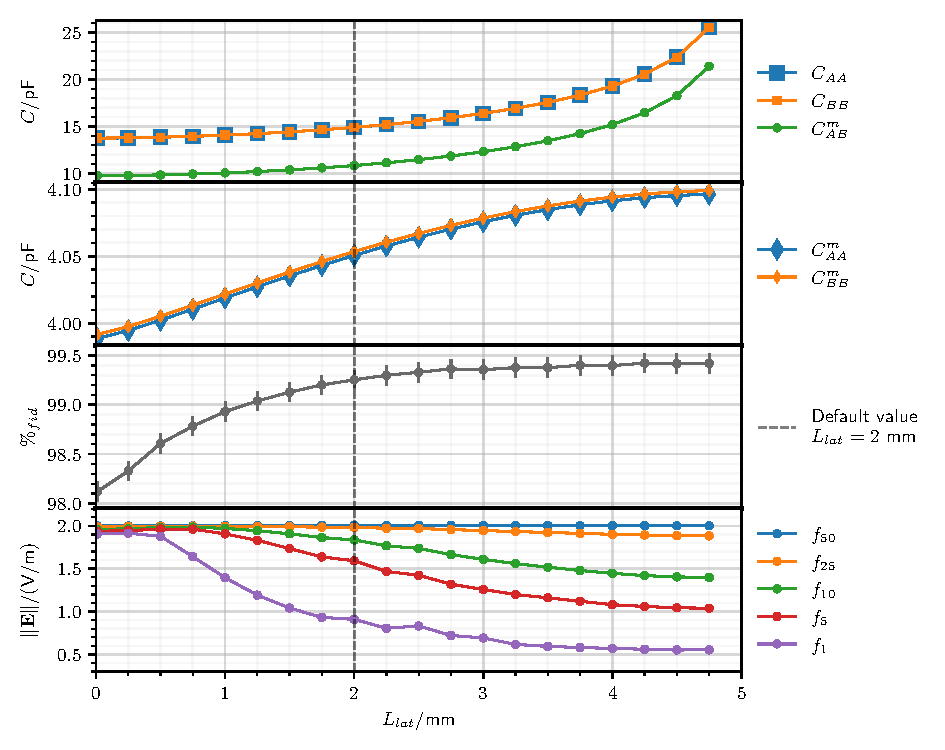
\includegraphics[scale=1]{Figures/ElectrodesScan/capacitance_fiducial_corner_length.pdf}
\caption{Scan over the corner length $L_{lat}$ for the PL38 design. The Maxwell and mutual capacitance terms, the percentage of fiducial volume and some percentiles of the electric field magnitude distribution are plotted. The default value $L_{lat}=\SI{2}{\mm}$ is represented by the dashed vertical line. Error bars for the capacitance terms are smaller than the marker size.}
\label{fig:capacitance-fiducial-corner-length}
\end{figure}

% Capacitance
As the corner length increases, the area of the top and bottom electrode grows. The self-capacitance terms $C_{XX}^m$ increases as the coupling with the ground rises but eventually seem to reach a plateau. The inter-electrode coupling term $C_{AB}^m$ increases with $L_{lat}$ especially at the highest values. Indeed, at high value of $L_{lat}$, the electrodes $A$ and $B$ are larger and also closer near the equator. As the corner length tends to \SI{5}{\mm}, with virtually touching top and bottom electrodes, the diagonal Maxwell terms diverge. On the same line, the electric field at the equator also diverge with ever closer top and bottom electrode, broadening the magnitude distribution toward higher values.
% Enorm
On the contrary, the electric field norm is lessened in the corners as the corner length increases and these low magnitude corner regions grow in size. A a result, the magnitude distribution expands toward lower values. This illustrated with the decreasing percentiles $f_1$ to $f_{25}$ on the figure \ref{fig:capacitance-fiducial-corner-length}. As a side note, the median magnitude of the electric field $f_{50}$ is constant for this scan. In the case of very short corner electrodes $L_{lat} \leq \SI{0.5}{\mm}$, the electric field norm is almost homogeneously equal to \SI{2}{\volt\per\meter} in the crystal.
{\color{red} [Comparison to enorm threshold, to do later.]}
% Fiducial
In fact, the electric field is almost uniform with the surface electric field lines bending towards the outside and eventually exiting the crystal, resulting in a loss of fiducial volume at low $L_{lat}$ values. With larger corner length, the fiducial volume fraction increases and caps at \SI{99.4}{\percent}. This limit is set by the streamlines are exiting the crystal at the surface of the central NTD hole.
% TWP
The total weighting potential on the bare lateral surface of the crystal increase slightly with the corner, starting from $0.94$ for a non existent corner $L_{lat}=\SI{0}{\mm}$ and reaching $0.99$ for a maximum corner length of \SI{4.8}{\mm}.   

% Conclusion
This scan over the corner length $L_{lat}$ features a performance balance between low capacitance terms and high electric field at low value and high fiducial volume at high corner length. As the variation on the fiducial volume is small, the control values points towards a performance optimization for the lowest value of the corner length $L_{lat}=\SI{0}{\mm}$. However, with this minimal value, the whole lateral surface of the germanium crystal is bare and prone to surface trapping due to the transversal trajectory of the electron in the crystal, as discussed in paragraph \ref{par:charge-drifting}. A conservative trade-off value is the default value $L_{lat}=\SI{2}{\mm}$.
{\color{red} [Comparison with experimental data with no corner electrode, REDN1 ?]}

% bonus observation 
% The non-diagonal capacitance term is drastically increased, which can be explained by the electrode A and B getting closer with the increasing corner length. For large corenr length, the area of the electrode facing the crystal are facing almost entirely the oppsite electrode and can only perceive the electric ground through the tight bare equator. This could explain the capping in the self-capacitance of A and B.
%In the corneres of the crystal, appearrance of growing low e norm region with slight divergence from the streamlines. Apparently not dangerous, because still a high enough enorm. (need confirmation)
%(danger fraction curve ?) 


\section{Specific to FID38}

This section is attributed to the FID design. Each paragraph presents the scan over a parameter. They are namely the width of the electrode rings $w_{Al}$, the radius of the central veto pad $r_{center}$, the distance between the edge of the crystal and the outermost planar electrode $w_{bare}$, the width of the outermost planar electrode $w_{outer}$, the equatorial distance $d_{eq}$, the polarization ratio $R_{veto}$ and the number of planar and lateral electrodes, $n_{plan}$ and $n_{lat}$ respectively. As the effects of the four latter parameters are heavily correlated, a paragraph is dedicated to the global scaling of the electrode density, scanning over selected configurations of this four parameters.


\subsection{Width of the Electrode Rings, $w_{Al}$}

The width $w_{Al}$ of the rings composing the electrodes is set by default to \SI{0.08}{\mm}. The scan is performed on a linear scale from \SIrange{0.5}{1.55}{\mm}. The results of the scan are presented in the figure \ref{fig:capacitance-fiducial-al-width}. They consist in graphs of the terms of the Maxwell and mutual capacitance matrices, the percentage of fiducial volume $\%_{fid}$ and some percentiles $f_x$ of the electric field magnitude distribution.

\begin{figure}[!h]
\centering
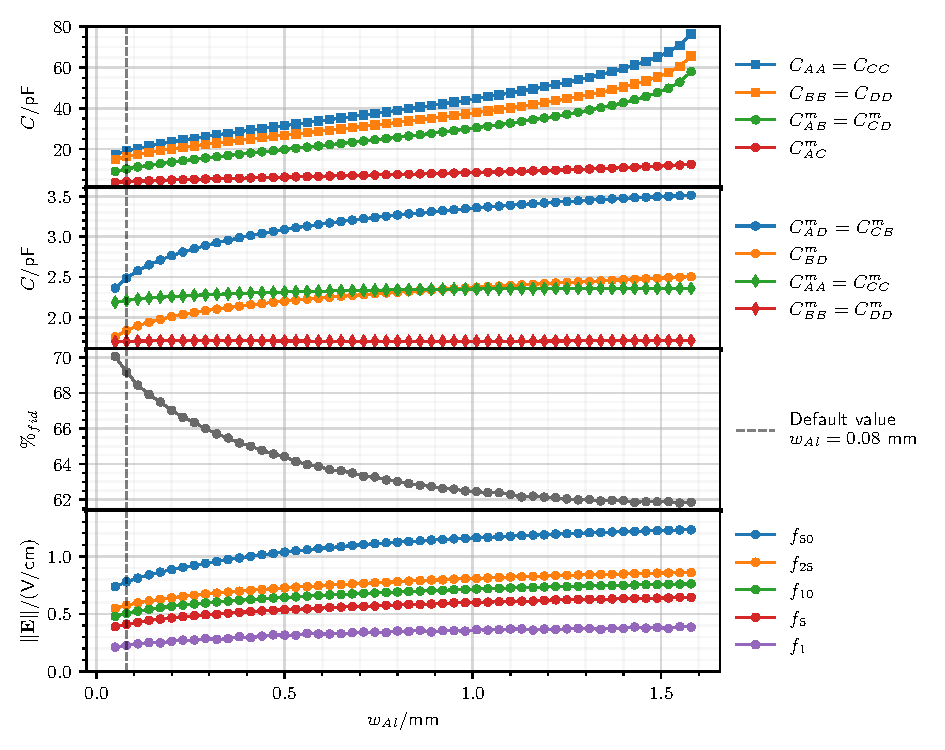
\includegraphics[scale=1]{Figures/ElectrodesScan/capacitance_fiducial_al_width.pdf}
\caption{Scan over the width of the electrode rings $w_{Al}$ for the FID38 design. The Maxwell and mutual capacitance terms, the percentage of fiducial volume and some percentiles of the electric field magnitude distribution over the crystal are plotted. The default value $w_{Al}=\SI{0.08}{\mm}$ is represented by the dashed vertical line. Error bars are smaller than the marker size.}
\label{fig:capacitance-fiducial-al-width}
\end{figure}

% Capacitance 
With a rising ring width $w_{Al}$, all electrodes gets closer from each other and their effective facing area increases. This explains the global augmentation of the capacitance with the ring width. The effect is most pronounced for the capacitive coupling term between same-sided veto and collect electrode $C_{AB}^m=C_{CD}^m$ which diverges as the electrode spacing tends to zero. The coupling between the two veto electrodes $C_{AC}^m$ moderately grows from the equatorial rings getting slightly closer. The remaining mutual term do not benefit from the decreasing spacing, and thus the increase induced by $w_{Al}$ is light. As sums of the mutual terms, the diagonal Maxwell capacitance term follows the increasing trend with diverging for high ring width.
% Fiducial
There is a significant decrease of the fiducial volume with increasing ring width until approximately \SI{1}{\mm} where a lower cap seems to be reached. As the electrode ring gets larger, the veto regions gain in depth, reducing the fiducial volume. 
% Enorm
This is consistent with the position of the low electric field magnitude regions under the veto rings getting deeper into the crystal. As the veto and collect electrodes are getting closer, the electric field in the veto regions greatly increase and grows more gently in the bulk of the crystal. Overall, the electric field norm globally rise with the ring width $w_{Al}$ and approach a plateau at high value. {\color{red} [Comparison to enorm threshold, to do later.]}
 %TWP
With higher $w_{Al}$, the total weighting potential on bare germanium surface slightly rise from $0.94$ for the thinnest ring, to $0.98$ for the largest ring possible before contact. Indeed, the grounded chassis is overshadowed by the large electrode and receive a reduced induced signal from the drifting electric charge.

% Conclusion
The results of the scan show that a high width for the electrode rings is very detrimental to the capacitance terms and the fiducial volume. The only upside to large electrodes would be a guaranteed charge collection in the vicinity of the electrodes in response to a surplus of surface trapping. This issue has yet to be seen experimentally on any detector with thin electrodes. Moreover, as the electric field is amplified near the electrode though point effect, drifting electric charge in their vicinity is even less prone to transversal trajectory and surface trapping. As such, the FID38 design can have its best performance with the lowest ring width feasible, $w_{Al}=\SI{0.05}{\mm}$. At the moment, this parameter is subject to technical constraints as it is not possible to reliably deposit continuous aluminum ring of width inferior to $\SI{50}{\micro\meter}$. 


\subsection{Central Pad Radius, $r_{center}$}

In place of a hollow ring, the centers of the planar surfaces are occupied by a central disk pad of radius $r_{center}$. This central pad is attributed to the veto electrodes $A$ and $C$. Its default value is of\SI{0.25}{\mm}. While for the default FID38 design, the NTD thermal sensor is meant to be glued on a veto electrode ring, an alternative would be to use a large central for the NTD gluing. The scan is performed on a linear scale from \SIrange{0.08}{5}{\mm}. The results of the scan are presented in the figure \ref{fig:capacitance-fiducial-r-center}. They consist in graphs of the terms of the Maxwell $C_{XY}$ and mutual $C_{XY}^m$ capacitance matrices, the percentage of fiducial volume $\%_{fid}$ and some percentiles $f_x$ of the electric field magnitude distribution.

\begin{figure}
\centering
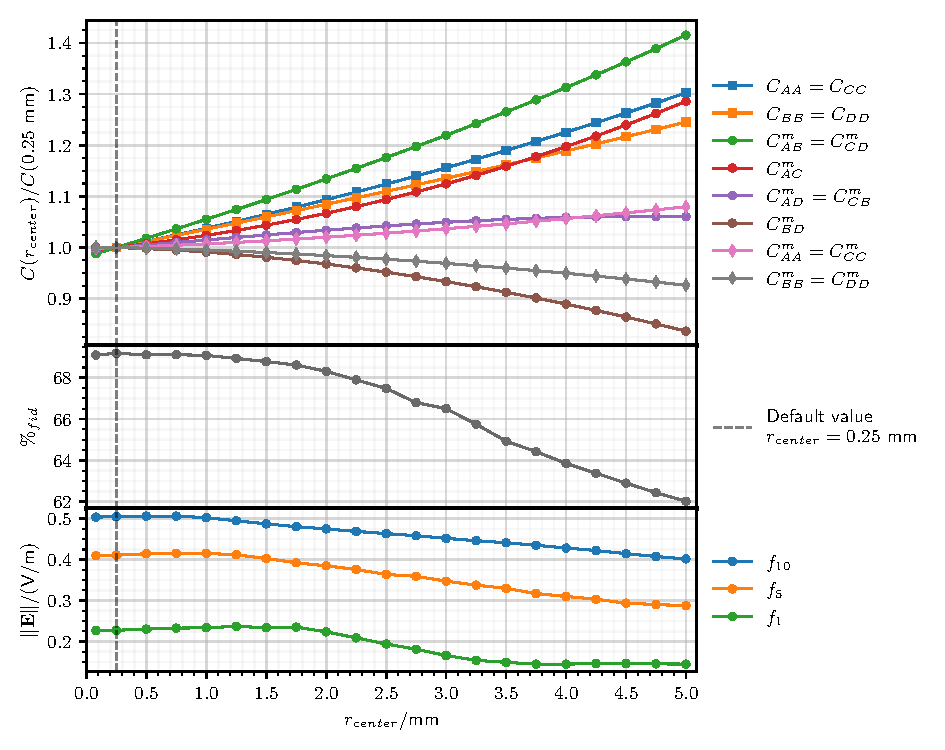
\includegraphics[scale=1]{Figures/ElectrodesScan/capacitance_fiducial_r_center.pdf}
\caption{Scan over the radius $r_{center}$ of the central planar aluminium pad for the FID38 design. The ratio of Maxwell and mutual capacitance terms, the percentage of fiducial volume and some percentiles of the electric field magnitude distribution are plotted. The default value $r_{center}=\SI{0.25}{\mm}$ is represented by the dashed vertical line. Error bars for the capacitance ratio are smaller than the marker size.}
\label{fig:capacitance-fiducial-r-center}
\end{figure}

As $r_{center}$ increase, the free planar space remaining for the other planar electrode rings decreases. This results in an increase in the planar ring density and a decrease in the planar ring spacing $d_{plan}$.
% Capacitance
The variation of the capacitance terms are modest for this scan. Therefore, the first plot of the figure \ref{fig:capacitance-fiducial-r-center} is the ratio of the capacitance terms over their value at default value \SI{0.25}{\mm}, where it is by definition equal to $1$. The two decreasing capacitance terms are the self-capacitance of the main collect electrode $B$ and $D$, as well as their coupling term $C_{BD}^m$. As the central veto pad grows, the innermost collect electrode rings are pushed away from the center. Apparently it emulates a loss of facing electrode area between the top collect electrode $B$ , the bottom collect electrode $D$ and the ground. The coupling term between the two veto electrode $C_{AC}^m$ is increased, which can be attributed to the growth of the central veto pad facing each other. The highest augmentation in capacitance is held by the coupling terms between same-sided veto and collect electrode $C_{AB}^m=C_{CD}^m$. It is explained by the lowered spacing between the planar electrode rings. As usual, the diagonal Maxwell capacitance terms $C_{XX}$ follows a similar trends to the dominating terms $C_{AB}^m=C_{CD}^m$.
% Fiducial
Concerning the fiducial volume, its percentage decreases with increasing central pad radius $r_{center}$. In fact, this loss is attributed to the growth of the veto region under the central pad. As this loss is centered on the rotational axis of the crystal, the loss is very light for low value of $r_{center}$. The remarkable value $r_{center} = \SI{1.5}{\mm}$, allowing for the gluing of a \SI{2 x 2}{\mm} NTD, shows a negligible decrease. However, the diminution in fiducial volume gets significant with higher radius.
% Enorm
Only the electric field norm in the center of the crystal is lowered by rising scanned parameter $r_{center}$. While the median $f_{50}$ of the magnitude distribution (not represented on figure \ref{fig:capacitance-fiducial-r-center}) is constant, the distribution is expanded towards lower values. This illustrated by the decreasing values of the percentiles $f_{1}$ to $f_{10}$. The explanation is the growth of the top and bottom low magnitude regions under the central veto pads which eventually merge for \SI{3}{\mm}. At this point, the electric field is nullified at the center of the crystal. With greater $r_{center}$, the electric field changes in direction with field lines connecting the top and bottom central veto pads.
{\color{red} [Comparison to enorm threshold, to do later.]}

% Conclusion
The result shows that all aspects of the performance of the ionization channel would profit from a small central pad radius $r_{center}$. The minimal value corresponds to the width of the electrode rings $r_{center}=\SI{0.08}{\mm}$. This study also demonstrates that at the cost of a small increase in capacitance, it would be viable to use a radius of \SI{1.5}{\mm} to fit a small NTD thermal sensor if need be.

% Bonus observation
%- twp: having a high $r_{center}$ boosts the twp in the crystal (center). As there is more veto electrode area, there is more signal induced on it, and less signal induced on the ground. (illustration ? twp under the veto electrode ? or just numbers)
%- however, with the lowest $r_{center}=\SI{0.08}{\mm}$, the depth of the veto region under the central pad is too shallow, and fiducial streamlines come very close the the surface. So $r_{center}=\SI{0.25}{\mm}$ is a good balance.


\subsection{Edge Veto Electrodes}

The outermost rings of the veto electrodes near the planar edge of the crystal are called the edge veto electrodes. Due their important role in shaping the electric field in the corners of the crystal and the constraints on the aluminum deposition at this location, the geometry of these corner veto electrodes calls for particular attention.
The constraints on the aluminum deposition depends on the techniques used. When using a deposition with mask, aluminum cannot be closer than \SI{0.3}{\mm} from the edge of the crystal. This results in the creation of a bare edge of width $w_{edge, bare}>=\geq \SI{0.3}{\mm}$. In the case of a deposition on the whole planar faces followed by photo-lithography, aluminum cannot be removed closer than \SI{1}{\mm} from the edge of the crystal. This technique thus results in large corner veto electrodes of width $w_{outer}\geq \SI{1}{\mm}$.
This section is separated in two studies, each investigating the two geometries for these edge veto electrodes.

% Width of Bare Germanium Edge, $w_{bare}$
% Width of Outer Veto Electrode Ring, $w_{outer}$

\subsubsection{Thin Outer Ring Spaced from the Crystal Edge, Scan over $w_{bare}$}

In this paragraph, we consider an aluminium deposition with a mask. The outermost planar ring is thin with a width of $w_{outer}=\SI{0.08}{\mm}$. This spacing between this outermost ring is spaced by a bare germanium surface of width $w_{bare}$ from the edge of the crystal. The scan is performed over the this bare germanium width $w_{bare}$ with a linear scale from \SIrange{0}{2}{\mm}. The reference configuration corresponds to the default FID38 design presented in the previous chapter \ref{ChapterElectrodes}. The edge veto electrodes are set to be as close as possible to the edge of the crystal with $w_{bare}=0.3mm$.
The results of the scan are presented in the figure \ref{fig:capacitance-fiducial-dead-edge}. They consist in graphs of the ratio of the terms of the Maxwell and mutual capacitance matrices, the percentage of fiducial volume $\%_{fid}$ and some percentiles $f_x$ of the electric field magnitude distribution. The constraint on the minimal feasible bare width $w_{bare} \geq \SI{0.3}{\mm}$ is represented by the shaded region.
  
\begin{figure}
\centering
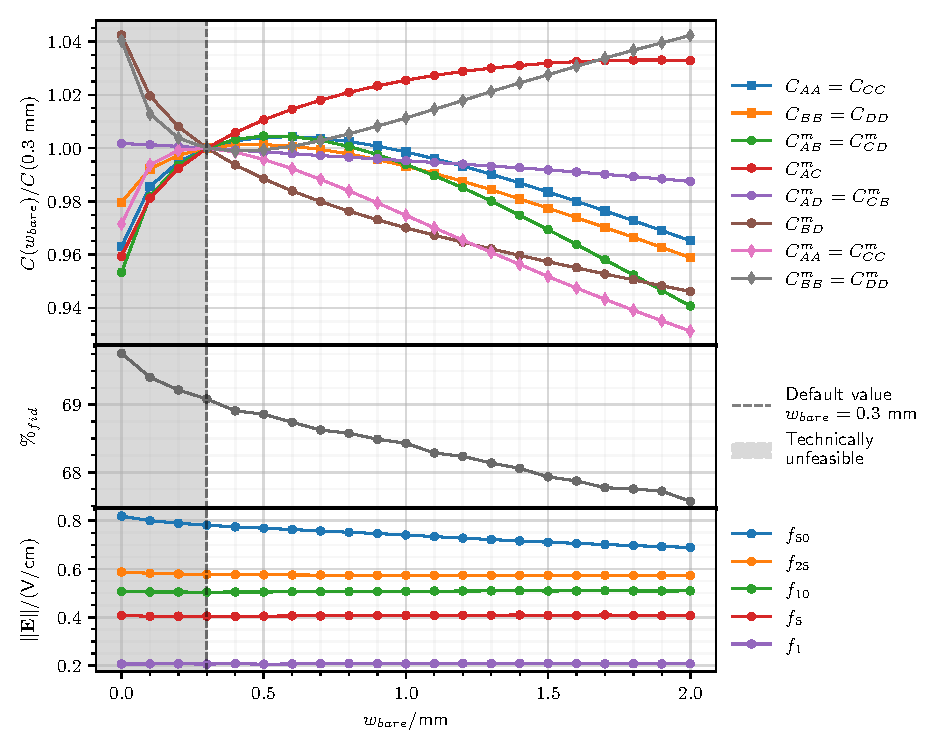
\includegraphics[scale=1]{Figures/ElectrodesScan/capacitance_fiducial_dead_edge.pdf}
\caption{Scan over the width of bare germanium $w_{bare}$ between the outermost planar electrode ring and the crystal edge for the FID38 design. The ratio of the Maxwell and mutual capacitance terms, the percentage of fiducial volume and some percentiles of the electric field magnitude distribution over the crystal volume are plotted. The capacitance term ratio is calculated with the default capacitance value as denominator. The default value $w_{bare}=\SI{0.3}{\mm}$ is represented by the dashed vertical line. A width strictly inferior to \SI{0.3}{\mm} is technically unfeasible which is represented by the shaded area. Error bars are smaller than the marker size.}
\label{fig:capacitance-fiducial-dead-edge}
\end{figure}

As the width of the bare edge increases, the free space available for the deposition of the other planar electrode ring diminishes. As a result, with the parameter $w_{bare}$ rising, the planar ring spacing $d_{plan}$ decreases.  
% Capacitance
The variation of the capacitance terms are very low, in the range of \SI{5}{\percent}, for this scan. Thus, the first plot of the figure \ref{fig:capacitance-fiducial-r-center} is the ratio of the capacitance terms over their value at default value \SI{0.3}{\mm}, where it is by definition equal to $1$. A large width $w_{bare}$ induces an increase in capacitance, due too the lowered planar spacing.
The coupling term of same-sided veto collect $C_{AB}^m=C_{CD}^m$ decreases for low or high value of $w_{bare}$ with a maximum near \SI{0.6}{\mm}. For low $w_{bare}$ value, the planar spacing $d_{plan}$ is high which explain the lowered capacitance between same-sided veto and collect electrode $C_{AB}^m=C_{CD}^m$. For high $w_{bare}$, the planar spacing $d_{plan}$ diminishes, explaining the maximum, but is eventually dominated by the loss of coupling due to the larger distance between the planar rings and the lateral rings. The coupling term of the veto electrodes $C_{AC}^m$ increases and cap with $w_{bare}$: the veto edge electrode rings are no longer overshadowed by the lateral collect electrodes. The coupling term of the collect electrodes $C_{BD}^m$ decreases with $w_{bare}$ as their effective facing area is lowered by their contracting rings. The self-capacitance of the veto electrodes $C_{AA}^m = C_{CC}^m$ shows a maximum around \SI{0.3}{\mm} (reason?). The self-capacitance of the collect electrodes $C_{BB}^m = C_{DD}^m$ features a minimum around \SI{0.4}{\mm} (reason?). In the end, the diagonal terms of the Maxwell capacitance matrix $C_{XX}$ follows the trend of the dominant term $C_{AB}^m$ with smooth maximum between 
\SI{0.3}{\mm} and \SI{0.8}{\mm}.
% Fiducial
The bare germanium width slightly changes the shape of the electric field lines in the crystal corners. The veto regions are growing near the corners As a result, the fiducial volume is slightly decreasing with rising $w_{bare}$. We also note that with $w_{bare} > \SI{0}{\mm}$, there is appearance of the corner regions with uncertain charge collection, as discussed in the previous chapter \ref{ChapterElectrodes}. {\color{red} [Estimation of the Corners regions volume ?]}
% TWP
In the vicinity if the corners, the total weighting potential on the surface is lighlty affected. I decreases from $0.94$ at default configuration to $0.86$ with $w_{bare} = \SI{2}{\mm}$.
% Enorm
With a high $w_{bare}$ corner regions feature a lower than default electric field norm. As a result, the median of the magnitude distribution in the crystal volume decreases moderately. However, the lower percentiles $f_{x \leq 25}$ remains stable.

% Conclusion
For the best value considering the bare width, the results points towards the minimal $w_{bare} = \SI{0}{\mm}$ which is not currently feasible. A high $w_{bare}$ would reduce marginally the capacitance values at the cost of creating large corner regions with uncontrolled charge collection. All in all, the minimum technically feasible value $w_{bare}=\SI{0.3}{\mm}$ seems to be the best configuration for a thin outer veto electrode ring.


\subsubsection{Large Outer Ring on the Crystal Edge, Scan over $w_{outer}$}

We now consider an aluminium deposition on the full planar surface followed by photo-lithography. The outermost planar ring is in contact with the crystal edge with $w_{bare}=\SI{0}{\mm}$. This outermost ring is large with a width of $w_{outer}$ which is scanned over in this paragraph. The scan is performed over a linear scale from \SIrange{0}{2}{\mm}. The results of the scan are presented in the figure \ref{fig:capacitance-fiducial-full-edge}. They consist in graphs of the ratio of the terms of the Maxwell and mutual capacitance matrices, the percentage of fiducial volume $\%_{fid}$ and some percentiles $f_x$ of the electric field magnitude distribution. The constraint on the minimal feasible outer ring width $w_{bare} \geq \SI{1}{\mm}$ is represented by the shaded region. For the capacitance ratio, the reference configuration corresponds to the minimal width of $\SI{1}{\mm}$.

\begin{figure}
\centering
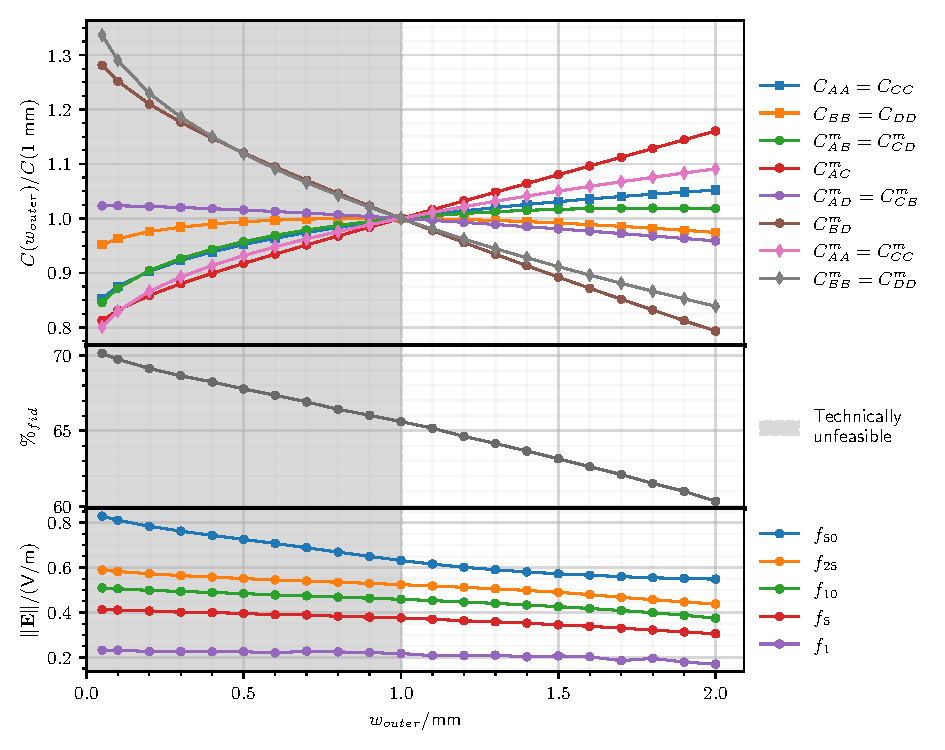
\includegraphics[scale=1]{Figures/ElectrodesScan/capacitance_fiducial_full_edge.pdf}
\caption{Scan over the width of the outermost veto electrode ring $w_{outer}$ for the FID38 design. The ratio of the Maxwell and mutual capacitance terms, the percentage of fiducial volume and some percentiles of the electric field magnitude distribution over the crystal volume are plotted. The capacitance term ratio is calculated with the capacitance value at $w_{outer}=\SI{1}{\mm}$ as reference. A width strictly inferior to \SI{1}{\mm} is technically unfeasible which is represented by the shaded area. Error bars are smaller than the marker size.}
\label{fig:capacitance-fiducial-full-edge}
\end{figure}

As the width of the outer ring $w_{outer}$ increases, the free space available for the deposition of the other planar electrode ring diminishes. As a result, with the parameter $w_{outer}$ rising, the planar ring spacing $d_{plan}$ decreases.
% Capacitance
The influence of $w_{outer}$ on the capacitance terms is subtle. The result on capacitance are presented in the first plot of the figure \ref{fig:capacitance-fiducial-r-center} as ratio of the capacitance terms over their reference value for \SI{1}{\mm}, where it is by definition equal to $1$. The dominant term $C_{AB}^m=C_{CD}^m$ increases and reach a cap near \SI{1.5}{\mm} (reason?). The collect coupling term $C_{BD}^m$ decreases significantly.  Indeed, the collect electrodes are more and more in regard of the growing outer veto electrode which overshadow the influence of the opposite collecting electrode. The self-capacitance of the collect electrode $C_{BB}^m=C_{DD}^m$ decreases as the collect electrode rings shrink, emulating a loss of effective area for capacitive coupling with the ground. Following the trend of $C_{AC}^m$, the diagonal veto term $C_{AA} = C_{CC}$ of the Maxwell matrix increase and cap. The diagonal collect term $C_{BB} = C_{DD}$ of the Maxwell matrix remains pretty constant with a maximum at the default value \SI{1}{\mm}. The increasing trends of the veto collect coupling term $C_{AB}^m$ is mitigated by the trends of the other capacitance relative to the collect electrodes.
% Fiducial
The fiducial volume decreases with $w_{outer}$ because the veto region on the corners are getting bigger. As this growth in veto volume is located on the periphery of the crystal, it represents a significant decreases in volume.
% enorm
This also in agreement with the observation on the electric field. The low electric field norm regions situated below the outer veto electrode rings gets deeper and closer to the center with increasing outer width $w_{outer}$. Consequently, the bulk and surface region see their electric field magnitude globally decrease. This is illustrated by all the diminishing percentiles of the magnitude distribution. {\color{red} [Comparison to enorm threshold, to do later.]}

%Conclusion
The influence on the capacitance term is noticeable but not that significant. On the contrary, the fiducial volume is significantly impacted by the parameter $w_{outer}$. The best design solution would be to have a minimal width of $w_{outer}=\SI{0}{\mm}$ which is not technically feasible. Thus, for now, the best configuration would be to consider the lowest possible width of \SI{1}{\mm}.


\subsubsection{Comparing the Two Geometries}

With the insights gathered from the scan over $w_{bare}$ and $w_{outer}$, we discuss and compare the two geometries fro the edge veto electrodes. Both studies points towards the same ideal best solution: having a thin $w_{Al} = \SI{0.08}{\mm}$ outer veto electrode ring in contact $w_{bare}=\SI{0}{\mm}$ with the edge of the crystal for low capacitance values and higher fiducial volume. This configuration is not possible technically for now. Now, comparing the best compromise offered by the two next best geometries:
\begin{itemize}
	\item Thin Outer Ring Spaced from the Crystal Edge, $\{ w_{outer} = \SI{0.08}{\mm}, w_{bare} = \SI{0.3}{\mm} \}$
	\item Large Outer Ring on the Crystal Edge, $\{ w_{outer} = \SI{1}{\mm}, w_{bare} = \SI{0}{\mm} \}$
\end{itemize}

{\color{red} [table with capacitance values and fiducial volume, and other bonus category: danger zone volume !]}

Conclusion: thin electrode favored for now, but backup design is with large electrode for now.
Waiting for experimentations with danger corner region to have more insights on the danger corner region.


\subsection{Equatorial Distance, $d_{eq}$}
\label{par:equatorial-distance}

The equatorial distance $d_{equator}$ corresponds to the distance between the two veto electrodes on the middle of the lateral surface of the crystal. By default, it is set to \SI{2}{\mm}. The scan is performed over a linear scale from \SIrange{0.2}{6}{\mm}. The results of the scan are presented in the figure \ref{fig:capacitance-fiducial-equatorial-distance}. They consist in graphs of the terms of the Maxwell $C_{XX}$ and mutual $X_{XY}^m$ capacitance matrices, the percentage of fiducial volume $\%_{fid}$ and some percentiles $f_x$ of the electric field magnitude distribution. 

\begin{figure}
\centering
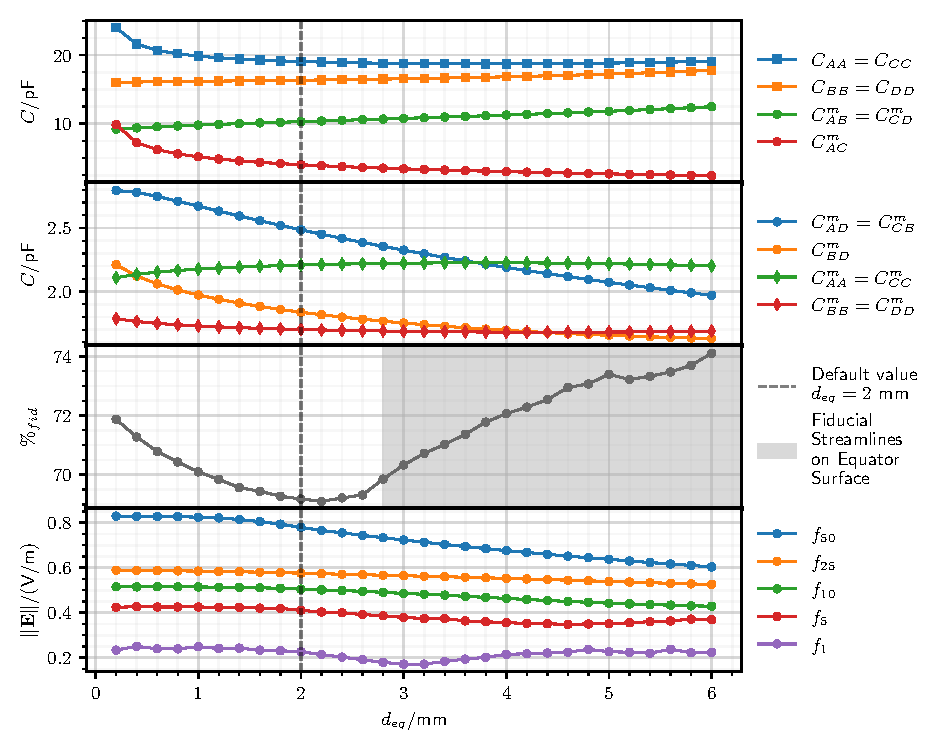
\includegraphics[scale=1]{Figures/ElectrodesScan/capacitance_fiducial_equatorial_distance.pdf}
\caption{Scan over the equatorial distance $d_{eq}$ of the FID38 design. The Maxwell and mutual capacitance terms, the percentage of fiducial volume ans some percentiles of the electric field magnitude distribution over the crystal volume are plotted. The default value $d_{eq}=\SI{2}{\mm}$ is represented by the dashed vertical line. Starting from \SI{2.8}{\mm}, fiducial streamlines are in contact with and exiting the crystal on the equatorial surface, this is represented by the shaded area. Error bars for the capacitance ratio are smaller than the marker size.}
\label{fig:capacitance-fiducial-equatorial-distance}
\end{figure}

As the equatorial distance $d_{eq}$ increases, the free lateral space available for the other lateral electrode rings diminishes. Thus, the lateral electrode density increases and the lateral spacing $d_{lat}$ shrinks. 
% Capacitance
This explains the augmentation of the capacitance term coupling same-sided veto and collect electrode $C_{AB}^m=C_{CD}^m$ at $d_{eq}$, which also fixes the trend of the diagonal Maxwell collect term $C_{BB}=C_{DD}$. On the contrary, the coupling term of the two veto electrodes $C_{AC}^m$ diverges as their separating distance $d_{eq}$ tends to zero. This remark is also valid at a lesser extent for the coupling term $C_{BD}^m$ and $C_{AD}^m = C_{BC}^m$,  as their associated separating distance on the lateral surface decreases with low value of $d_{eq}$. In the end, the diagonal Maxwell term of the veto electrodes $C_{AA} = C_{CC}$ features the diverges of the term $C_{AC}^m$ at low $d_{eq}$ and becomes almost constant with a very smooth minimum from \SIrange{2}{5}{\mm}.
% Fiducial
Scanning over the equatorial distance strongly affects the shape of the electric field lines near the equator. At low values, the equatorial region defined on scheme \ref{fig:sheme-fid38} is clearly defined. With increasing equatorial distance, the lateral veto regions grow deeper and fiducial volume as well as the equatorial region shrink. According to the fiducial graph, the fiducial fraction gets an minimum for \SI{2.2}{\mm}. Starting from \SI{2.8}{\mm}, there are no more equatorial field lines and the ever growing fraction of fiducial field lines comes into contact with the equatorial surface of the crystal. This transition is illustrated by the shaded on the figure \ref{fig:capacitance-fiducial-equatorial-distance} featuring a rise in the fiducial volume. This configuration of the field lines nullify the use of the FID design aiming at discarding any surface event. Any surface event happening in the vicinity of the equator would not be tagged by the veto electrodes and would be heavily prone to surface trapping on the equator surface.
% Enorm
In this regime of high $d_{eq}$ values, the low electric field magnitude regions associated with the veto equatorial electrodes are large and covers a majority of the peripheral volume of the crystal. As a result, the median $f_{50}$ of the magnitude distribution shifts towards lower values. However, the lower percentiles $f_{x \leq 25}$ are less affected.
{\color{red} [Comparison to enorm threshold, to do later.]}
% TWP
Concerning the generation of the signal for electric charge possibly trapped on the equatorial surface, the total weighting potential is negatively affected by the rising $d_{eq}$ with a value of $0.99$ of the equator at $d_{eq}=\SI{0.2}{\mm}$ dropping to $0.90$ with the maximal equatorial distance of \SI{6}{\mm}.

% Conclusion
In the end, by considering the shape of the electric field, the FID38 design can only operate with an equatorial distance $d_{eq}$ from \SIrange{0.2}{2.6}{\mm}. At the lowest distance, a very low \SI{2}{\percent} increase in fiducial volume in obtained at the cost significantly increased capacitance. A good balance is found for an equatorial volume in the range from \SIrange{1.2}{2.6}{\mm}.
% Disclaimer
The influence of the equatorial distance $d_{eq}$ on the capacitance terms and the electric field strongly depends on the values of the parameters $\{R_{veto}, n_{plan}, n_{lat} \}$. In particular, the behavior of the electric field lines near the equator for $d_{eq} \geq \SI{2.8}{\mm}$ can be mitigated by  judiciously chosen polarization ratio value different from the default one $R_{veto} = \num{0.25}$. The study of the interaction between these four parameters is presented in the later paragraph \ref{par:global-density}.

% bonus observation
% - enorm hist: there is a uniformisation of the efield norm in the crystal as the distance is getting bigger. Uniformization towards main peak. (enorm distribution std and mode curve ?)
%Maybe, 1mm appears to be the optimum for the default parameters used for FID38, and there may be another optimal values for different parameters.


\subsection{Polarization Ratio, $R_{veto}$}
\label{par:veto-ratio}

The polarization ratio $R_{veto}$ fixes the electric potential of the veto electrodes in regard to the polarization of the collect electrodes. This parameter is introduced in the equation \ref{eq:veto-ratio} in the previous chapter \ref{ChapterElectrodes} where its default value for the FID38 design is set to $0.25$. The scan is performed over a linear scale from \SIrange{-1}{1}{}. The results of the scan are presented in the figure \ref{fig:capacitance-fiducial-veto-ratio}. They consist in graphs of the percentage of fiducial volume $\%_{fid}$ and some percentiles $f_x$ of the electric field magnitude distribution. 

\begin{figure}
\centering
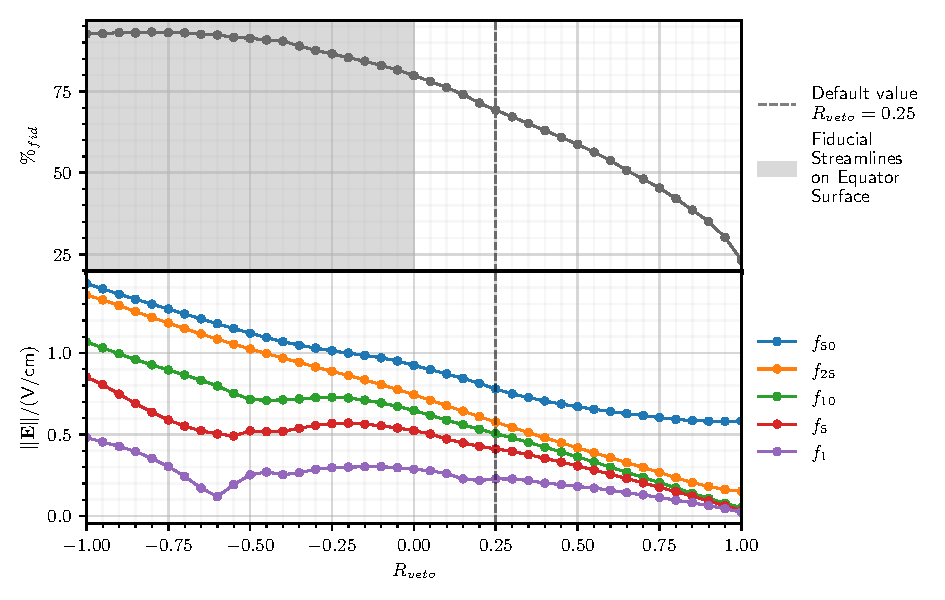
\includegraphics[scale=1]{Figures/ElectrodesScan/capacitance_fiducial_veto_ratio.pdf}
\caption{Scan over the polarization ratio $R_{veto}$ of the FID38 design. The percentage of fiducial volume and some percentiles of the electric field magnitude distribution over the crystal volume are plotted. The default value $R_{veto}=\SI{0.25}{\mm}$ is represented by the dashed vertical line. For values lower than $0.2$, electric field lines are incompatible with a correct operation of the FID detector. This is represented by the shaded area. Error bars for the capacitance ratio are smaller than the marker size.}
\label{fig:capacitance-fiducial-veto-ratio}
\end{figure}

% unaffected
As the polarization ratio $R_{veto}$ only sets the electric potential of the electrodes and leaves intact the geometry of the electrodes, the capacitance matrices as well as the weighting potentials remain unaffected for this study.
% Fiducial
The fiducial volume fraction decreases with $R_{veto}$ and reaches a maximum of about \SI{95}{\percent}for $R_{veto}=-1$. This configuration (not the only value when this happens, for other ratio too) corresponds to an electric field very similar to a planar detector (like the PL38 design) where same-sided electrodes are equally collecting drifting charges. This mode of operation (discussed previously in chapter \ref{ChapterElectrodes}, paragraph?) is not compatible with the tagging of the surface events.
The fiducial volume fraction reaches a minimum for $R_{veto}=1$ when $V_A = V_D = -V_B = -V_C$. In this configuration, the electric field in the bulk of the crystal is nullified, if not slightly reverses due to the higher total number of veto electrode rings.
For $R_{veto} \leq -0.3$, the FID38 detector is in a planar-like polarization. There are no veto region. All the electrodes behaves as collecting electrodes.
For $R_{veto} \geq -0.3$, shallow veto regions appears. Small region of low electric field norm are presents under the veto electrodes rings. However, the electric field in the equatorial region has the same direction as the electric field in the bulk region.
For $R_{veto} \geq 0$, veto regions along with the low $|\vec{E}|$ regions associated are getting deeper. The equatorial volume has vanished as the fiducial streamlines are now touching the crystal equatorial surface. 
For $R_{veto} \leq 0.2$, the equatorial volume is present with an electric field of opposite direction to the one in the bulk region. The electric field structure is standard for a FID operation as presented in the scheme \ref{fig:scheme-fid38}. As the polarization ratio $R_{veto}$ increases, the veto regions and the equatorial region grow in size, reducing the fiducial volume. Eventually, the regions of low electric field magnitude under the veto electrodes are big and deep enough to merge and hold the bulk of the crystal.
% Enorm
The magnitude of the electric field in the bulk of the crystal decreases with the rising $R_{veto}$. Far from the electrodes, the interleaved same-sided veto and collect electrode rings appears to have the influence of an equivalent planar electrode of electric potential $V=\frac{V_B + V_A}{2}$ and so the perceived electric field norm in the bulk is $E = \frac{V_B + V_A - V_D - V_C}{2 H_{Ge}}=...$ (this calculation should appears when introducing the norm of the electric field and discussing the figure at default value. The calculation explain the phenomenon observed now during the scan over $R_{veto}$).
{\color{red} [Comparison to enorm threshold, to do later.]}

% Conclusion
$R_{veto}$ should be high enough to be in a polarization mode compatible with the tagging of surface events, while being low enough to keep a good fiducial volume fraction.
The lower threshold on a valid $R_{veto}$ is apparently imposed by the existence of an equatorial region with an electric field of opposite direction to the bulk electric field. Is it really necessary to have opposite direction ? Yes, or else, a lot of bulk events would deposit some signal on the equatorial rings. So, we have a hard constraint of $R_{veto} > 0$. In order to have the actual existence of the equatorial region, the influence of the veto equatorial rings should be greater than the collect ring, that is to say, fiducial streamlines should not contact with the equatorial surface. the obvious solution is to increases the polarization ratio $R_{veto}$ at the detriment of the fiducial volume.
It might also be possible to tweak the equatorial distance $d_{eq}$ to mitigate the low electric potential of the veto electrode.
% Disclaimer
The influence of the polarization ratio $R_{veto}$ on the electric field strongly depends on the values of the parameters $\{R_{veto}, n_{plan}, n_{lat} \}$. In particular, the behavior of the electric field lines near the equator for $R_{veto} \leq \SI{0}{}$ can be compensated by adapting the value of the equatorial distance $d_{eq}$ instead of fixing it to its default value of \SI{2}{\mm}. The study of the interaction between these four parameters is presented in the later paragraph \ref{par:global-density}.

\subsection{Number of Planar Electrode Rings, $n_{plan}$}
\label{par:n-plan}

The collect and veto electrodes of the FID38 design consists in concentric aluminium rings deposited on the planar and lateral surface of the germanium crystal. The number of concentric planar rings, including the central veto pad, on single planar surface corresponds to the parameter $n_{plan}$.
As the FID38 design is based on having the collect electrodes $B,D$ interleaved with the veto electrodes $A,C$, it is necessary to assign the central aluminium pad and the outermost ring to the veto electrodes as was discussed in paragraph ref(TODO)). Therefore, $n_{plan}$ is an odd integer. As the electrode rings are evenly spread on the free planar surface of the crystal of fixed radius $R_{Ge}=\SI{15}{\mm}$, their number $n_{plan}$ sets the planar ring spacing $d_{plan}$ and their density on the surface.
By default, $n_{plan}$ is set to $7$ which corresponds to the spacing between the planar rings to $d_{plan}=\SI{2.40}{\mm}$.  The scan is performed for the values \SIlist{3;5;7;9;11}{}. The results of the scan are presented in the figure \ref{fig:capacitance-fiducial-n-top}. They consist in graphs of the percentage of Maxwell and mutual capacitance terms and the percentage of fiducial volume $\%_{fid}$.

\begin{figure}
\centering
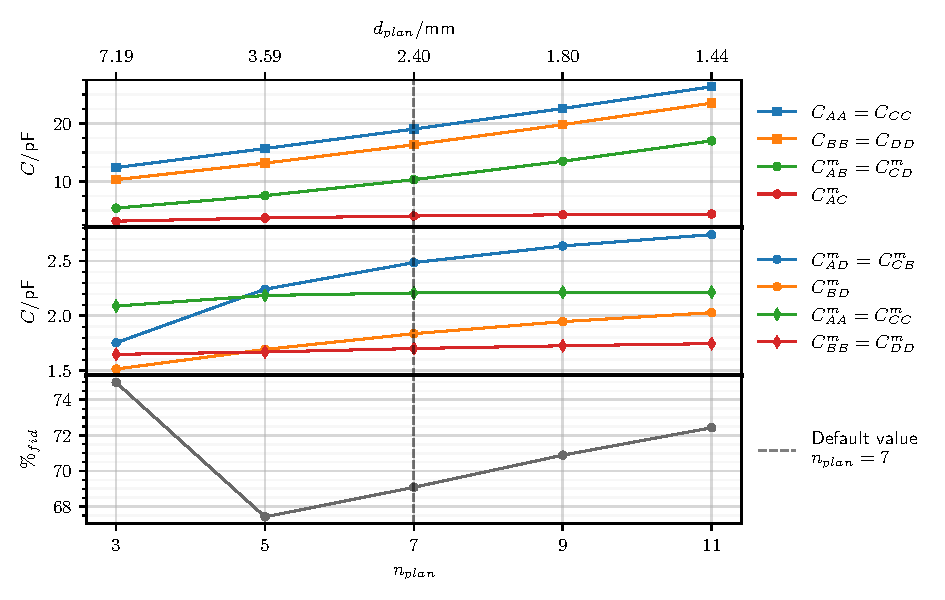
\includegraphics[scale=1]{Figures/ElectrodesScan/capacitance_fiducial_n_top.pdf}
\caption{Scan over the number of planar electrode rings $n_{plan}$. The Maxwell and mutual capacitance terms and percentage of fiducial volume are plotted. The default value $n_{plan}=7$ is represented by the dashed vertical line. The parameter $n_{plan}$ is restricted to odd integers in order to assign the central pads and the outermost rings to the veto electrodes $A$ and $C$. The corresponding values of spacing between planar rings $d_{plan}$ are mentioned at the top of the graph. Error bars are smaller than the marker size.}
\label{fig:capacitance-fiducial-n-top}
\end{figure}

% Capacitance
According to equation \ref{eq:planar-spacing}, the planar spacing $d_{plan}$ is proportional to the inverse of the number of planar ring $n_{plan}$. A higher number of aluminium rings emulates a higher area available for capacitive coupling and also decrease the distance between the electrodes. As a result, all coupling term increase with the number of planar ring. Attenuated variation are observed for the terms $C_{AC}^m$ and $C_{XX}^m$ as the distance to the chassis  and the equatorial distance between the veto electrodes $A$ and $C$ remain the same. As usual, the variation diagonal Maxwell term are dominated by the trend of the terms $C_{AB}^m=C_{CD}^m$.
% Fiducial streamlines
Apart from the first point, the fiducial volume grows with an increasing number of planar rings. This is explained by a loss of depth and volume of the surface veto regions. 
% Anomaly, first point
The minimal number of planar electrodes $n_{plan}=3$ shows a particular behavior. For this configuration, the fiducial volume is maximal. However, a lot of fiducial streamlines are almost parallel to the planar surface, which could be problematic with the transversal trajectory of the electrons. Moreover, the regions of low electric field magnitude associated to the veto electrodes are in contact with the planar surface, surely resulting in high fraction of trapped event on the planar surface. 

% Conclusion
The number of planar electrode rings $n_{plan}$ can be used to have a better control on the shape of the electric field with a higher fiducial volume at the expense of a significant increase in capacitance. Alone, this parameter mainly affect the behavior near the center of the detector as the number of lateral electrode ring $n_{lat}$ is fixed. Its effect on the fiducial volume is strongly correlated with the influence of the polarization ratio $r_{veto}$. In the later paragraph \ref{par:global-density}, the number of planar ring $n_{plan}$ is scanned over with adapted number of lateral electrode $n_{lat}$ and the polarization ratio $R_{veto}$.
% Disclaimer
The effect of number of planar ring $n_{plan}$ on the capacitance and electric field strongly depends on the values of the parameters $\{n_{lat}, R_{veto}, d_{eq}\}$. In particular, it is more efficient to have a similar ring density on the planar and lateral surface in order to lower the capacitive cost of shaping the electric field in the crystal. The study of the interaction between these four parameters is presented in the later paragraph \ref{par:global-density}.


\subsection{Number of Lateral Electrode Rings, $n_{lat}$}
\label{par:n-lat}

The collect and veto electrodes of the FID38 design consists in concentric aluminium rings deposited on the planar and lateral surface of the germanium crystal. The lateral surface is divided in two part, top and bottom, separated by the equator line of the crystal. In the top part of the lateral surface are located the aluminium attributed to the electrode $A$ and $B$. In the bottom part of the lateral surface are located the aluminium attributed to the electrode $C$ and $D$. The parameter $n_{lat}$ corresponds to the number of lateral ring in either the top or the bottom part of the lateral surface. The total number aluminium rings on the whole lateral surface is therefore $2 n_{lat}$. As the FID38 design is based on having the collect electrodes $B,D$ interleaved with the veto electrodes $A,C$, it is necessary to assign the ring closest to the equator to the veto electrodes $A$ and $C$ and the ring closest to the edge of the crystal to the collect electrodes $B$ and $D$. As such, $n_{lat}$ is an even integer. As the electrode rings are evenly spread on the free lateral surface of the crystal of fixed height $H_{Ge}=\SI{10}{\mm}$, the parameter $n_{lat}$ sets the lateral ring spacing $d_{lat}$ and their density on the surface. By default, $n_{lateral}$ is set to $2$ which corresponds a spacing between the lateral rings of $d_{lat}=\SI{1.98}{\mm}$.  The scan is performed for the values \SIlist{2; 4; 6; 8}{}. The results of the scan are presented in the figure \ref{fig:capacitance-fiducial-n-top}. They consist in graphs of the percentage of Maxwell and mutual capacitance terms and the percentage of fiducial volume $\%_{fid}$.

\begin{figure}
\centering
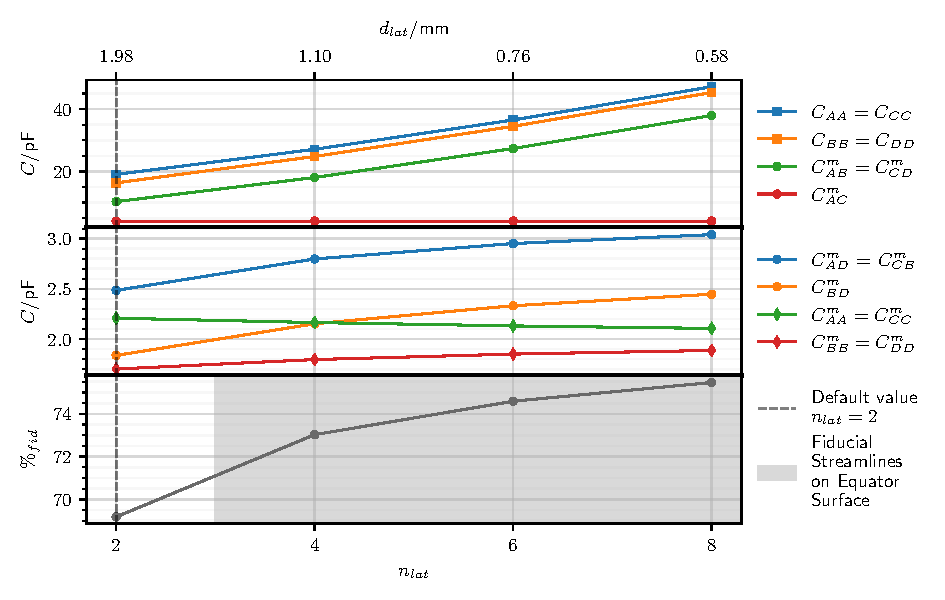
\includegraphics[scale=1]{Figures/ElectrodesScan/capacitance_fiducial_n_lat.pdf}
\caption{Scan over the number of planar electrode rings $n_{lat}$. The Maxwell and mutual capacitance terms and percentage of fiducial volume are plotted. The default value $n_{lat}=2$ is represented by the dashed vertical line. The parameter $n_{lat}$ is restricted to even integers in order to equatorial ring to the veto electrodes and the ring closest to the crystal edge to the collect electrodes. The corresponding values of spacing between lateral rings $d_{lat}$ are mentioned at the top of the graph. Error bars are smaller than the marker size.}
\label{fig:capacitance-fiducial-n-lat}
\end{figure}

% Similar to n-plan
The observations resulting from the scan over $n_{lat}$ are very similar to the ones from the scan over the number of planar rings $n_{plan}$ presented in the previous paragraph \ref{par:n-plan}, with a few differences. With an increasing number of lateral rings, almost all the capacitance terms increase and the fiducial volume grows.
% loss of equatorial volume
For this scan, the increasing fiducial volume is associated to the shrinking of the surface veto regions, the parameter $n_{lat}$ does not affect much the center ($r\lesssim\SI{10}{\mm}$) of the crystal. However, this growth is also associated to the disappearance of the equatorial volume. Indeed, for $n_{lat} \leq 4$, fiducial streamlines comes into contact with the equatorial surface and leave the crystal. These configurations are therefore not compatible with the correct FID operation.

% Conclusion
The number of planar electrode rings $n_{plan}$ can be used to have a better control on the shape of the electric field with a higher fiducial volume at the expense of a significant increase in capacitance. Alone, this parameter mainly affect the behavior on the periphery of the detector as the number of planar electrode ring $n_{plan}$ is fixed. The effect of the number of lateral rings $n_{lat}$ on the capacitance and electric field strongly depends on the values of the parameters $\{n_{plan}, R_{veto}, d_{eq}\}$. In particular, the behavior of the electric field lines for $n_{lat} \geq 4$ can be suppressed with an adaptation of the equatorial distance $d_{eq}$ and the polarization ratio $R_{veto}$. The study of the interaction between these four parameters is presented in the later paragraph \ref{par:global-density}.

\subsection{Global Density of the Electrode Rings, $\{n_{plan}, n_{lat}, R_{veto}, d_{eq}\}$}
\label{par:global-density}

The four previous paragraph \ref{par:equatorial-distance} to \ref{par:n-lat} are dedicated to uni-dimensional scan over the parameters $\{n_{plan}, n_{lat}, R_{veto}, d_{eq}\}$. In this paragraph, these four parameters are scanned over in unison in order to emulate an increasing and uniform global density of the electrode rings with adapted polarization.
% Choice of the n-plna an d n-lat
The parameters $\{n_{plan}, n_{lat} \}$ participate in shaping the electric field at the cost of heightened capacitance term, in the center and in the periphery of the crystal respectively. Performances of the ionization channel are uniform in the whole volume of the crystal if the electric field demonstrate homogeneous properties in the crystal. Namely, the density of the electrode rings should be equivalent on the planar surfaces and the lateral surfaces. Thus, the parameters $\{n_{plan}, n_{lat} \}$ are chosen such that the planar $d_{plan}$ and lateral $d_{lat}$ spacing are as close as possible. It happens that the same values of $n_{plan}$ or $n_{lat}$ can be used in multiple configurations. Nevertheless, the result are presented with a monotonically increasing number of total electrodes rings on the detector.
{\color{red} [Table with n-plan, n-lat , d-plan, d-lat, is it needed ?]}
% Choice of the veto-ratio and equatorial distance
The results related to the three parameters $\{n_{lat}, R_{veto}, d_{eq}\}$ shows that a significant part of the parametric space is not compatible with a correct operation of the FID38 design with working surface event tagging. With judicious choice in the values of these parameters, it is possible to explore a viable part of the parametric space. As the parameter $n_{lat}$ is imposed by the choice of $n_{plan}$, the remaining parameters $R_{veto}$ and $d_{eq}$ should be considered as functions of the parameter $n_{lat}$. Considering the insights of the paragraph \ref{par:equatorial-distance} with the scan over the equatorial distance $d_{eq}$, the default value of of \SI{2}{\mm} is in the viable range and happen to be almost equal to default lateral spacing $d_{lat} = \SI{1.98}{\mm}$. A simplistic relation between $n_{lat}$ and the equatorial distance $d_{eq}$ is to have the later equal to the lateral spacing $d_{lat}$. The parameter $d_{lat}$ is deduced from the equation \ref{eq:lateral-spacing} which already features the equatorial distance $d_{eq}$. As to avoid the needlessly complex solution of a second-order polynomial equation, the equatorial distance is set to:
\begin{equation}
d_{eq} \left( n_{lat} \right) = \frac{H_{Ge}}{1 + 2 n_{lat}} \approx d_{lat}
\end{equation}
The last unfixed parameter is the polarization ratio $R_{veto}$. As discussed previously in paragraph \ref{par:equatorial-distance}, \ref{par:veto-ratio} and \ref{par:n-lat}, an existing equatorial region is necessary to the viable operation of an FID detector. The condition for the equatorial region to appear is that the electric field at the equator is nullified:
\begin{equation}
\bm{E}\left(z=\SI{0}{\mm}, r=\SI{15}{\mm} \right) \cdot \hat{\bm{z}} \geq 0
\end{equation}
The numerical resolution of this equation is surely possible with the electrostatic simulation. However, for the sake of simplicity in this explanatory scan, the polarization ratio is set the following empirical function:
\begin{equation}
R_{veto} = \left(1 + 4 \frac{d_{lat}}{d_{eq}} \right)^{-1} \approx 0.2
\end{equation}
With this choice on the three parameters $\{n_{lat}, R_{veto}, d_{eq}\}$, the equatorial regions exists and possesses enough volume to guarantee a good rejection of the surface events.

\begin{figure}
\centering
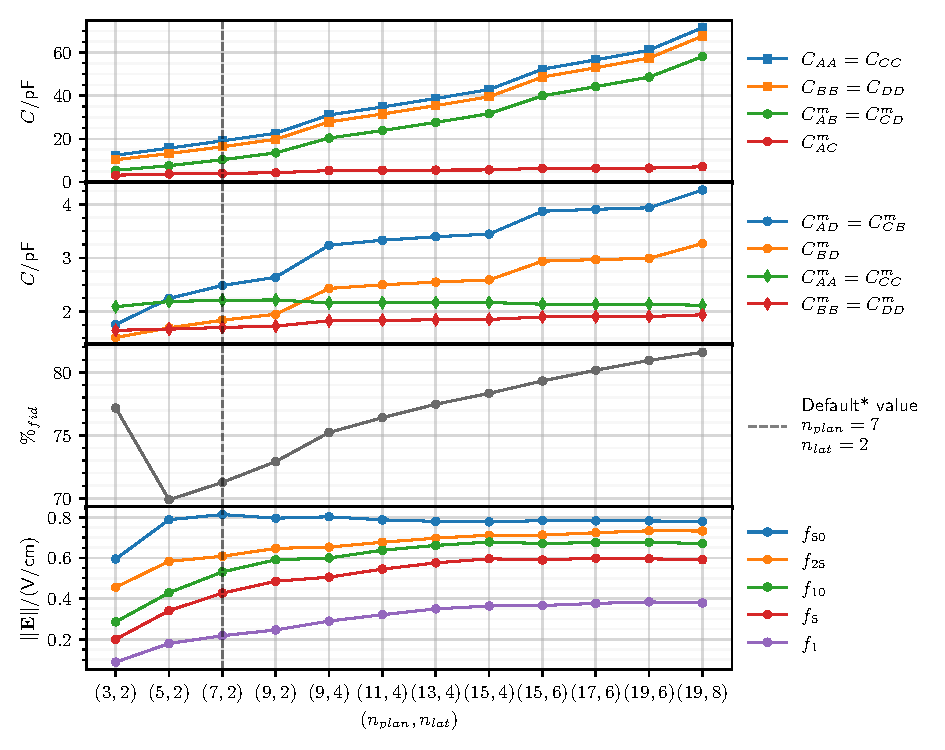
\includegraphics[scale=1]{Figures/ElectrodesScan/capacitance_fiducial_global_scale.pdf}
\caption{Scan over selected set of values for the parameters $\{n_{plan}, n_{lat}, R_{veto}, d_{eq}\}$ emulating an increasing homogeneous ring density for the FID38 design. The Maxwell and mutual capacitance terms, the percentage of fiducial volume and some percentiles of the electric field magnitude distribution over the crystal volume are plotted. The default configuration $(n_{plan}, n_{lat})=(7,2)$ is represented by the dashed vertical line, the polarization ratio $R_{veto}$ is different from the default configuration. Error bars are smaller than the marker size.}
\label{fig:capacitance-fiducial-global-scale}
\end{figure}

The simulation is ran with the considered set of values and the results are presented in the figure \ref{fig:capacitance-fiducial-global-scale}.  They consist in graphs of the terms of the Maxwell $C_{XX}$ and mutual $C_{XY}^m$ capacitance matrices, the percentage of fiducial volume $\%_{fid}$ and some percentiles $f_x$ of the electric field magnitude distribution over the crystal volume.
% Disclaimer default value
One should note that this value is close to the default value of the FID38 design, $R_{veto}=0.25$. As a result, the reference configurations on the graph $\left( n_{plan}, n_{lat} \right) = (7,2)$ demonstrates a slightly higher fiducial volume and global electric field than the default FID38 configuration presented in the previous chapter \ref{ChapterElectrodes}.

% Capacitance
Almost all the capacitance terms increase with the higher number of electrode rings. The coupling term related to same-sided vet and collect electrodes $C_{AB}^m=C_{CD}^m$ is greatly augmented as the planar and lateral spacing shrink. as this term is dominant in their calculation, the diagonal terms of the Maxwell matrix capacitance $C_{XX}$ follow the same trend. With a higher number of electrode rings, the effective area available for capacitive coupling is higher for all electrodes, which explains the growth of the terms $C_{BD}^m$ nad $C_{AD}^m=C_{CB}^m$ related to the coupling of electrode on opposite side. The self-capacitance terms are only slightly affected, and even decrease in the case of $C_{AA}^m=C_{CC}^m$. This can be associated with the overshadowing of the ground by the increasing number of rings which prevent further capacitive coupling with the electrodes.
% Fiducial
The fiducial volume demonstrate a behavior similar to the uni-dimensional scan over $n_{plan}$ and $n_{lat}$. Its percentage grows significantly with the number of electrodes, with a gain of \SI{12.5}{\percent} between the extrema. 
% Enorm
Indeed, with closer collect and veto electrodes, the veto regions lose depth and volume. However, the veto regions also gains in electric field norm with smaller low electric field magnitude regions. As a result, the electric field is more uniform in the crystal as illustrated by the stable median $f_{50}$ of the magnitude distribution and increasing lower percentiles.
{\color{red} [Comparison to enorm threshold, to do later.]}
% Particular point
The first point with $n_{plan} = 3$ remains an exception in the trend of the fiducial volume. Fiducial field lines occupy a larger portion of the volume at the cost of a low electric field magnitude in the planar veto regions. Indeed, all the percentiles of the magnitude distribution drop. Moreover, the discussion of paragraph \ref{par:n-plan} is still valid: with field lines parallel to the planar surface and low electric field, electrons are more prone to surface trapping because of their transversal trajectory in the germanium.
% TWP
For this particular configuration $(3,2)$, the total weighting potential on the surface of the crystal are about $0.84$. This value rise rapidly to reach the default value of $0.95$ and cap at $0.98$ for the maximal number of rings for the configuration $(19,8)$.

% Conclusion
With the exception of the first point $(3,2)$ demonstrating a potentially bad charge collection, an increasing density of the electrode rings yields a better control of the electric field with the growth of the fiducial volume at the expense of the global augmentation of the capacitance terms. The configuration $(5,2)$, $(7,2)$ and $(9,2)$ seems all viable and offer some flexibility on the FID38 design. With the lowest amount of electrodes $(5,2)$, the fiducial volume is relatively low, with a percentage of \SI{70}{\percent}, but features better resolution for the ionization channel thanks to lowered capacitance terms. The configuration $(9,2)$ loses in resolution, with a rough estimation of the loss of \SI{15}{\percent} by referring to the capacitance values, with a somewhat marginal gain in he percentage of theoretical fiducial volume of \SI{3}{\percent}.
